\chapter{Programming; Μα Γιατί;}
\label{chap:main-intro}
\section{Εισαγωγή}
Είμαστε σίγουροι ότι οι περισσότεροι από εσάς γεννηθήκατε ή
πρωτοχρησιμοποιήσατε υπολογιστή σε μια εποχή που οι δυνατότητες των
μηχανημάτων ήταν ήδη μεγάλες: θεωρείτε φυσιολογικό ο υπολογιστής σας να
παίζει video, να κατεβάζει ταινίες και μουσική από το Internet με μεγάλη
ταχύτητα και να τρέχει τα τελευταία 3D παιχνίδια (αφήνω κατά μέρος τους
εκβιασμούς στους γονείς σας να σας αγοράσουν την τελευταία και πανάκριβη
κάρτα γραφικών).

Θεωρείτε δεδομένο ότι ο υπολογιστής είναι κάτι που χειριζόμαστε με το
ποντίκι και οι νεότεροι από σας δεν έχουν δει ποτέ οθόνη με καθοδικό σωλήνα
(εκτός ίσως σε κανένα ξεχασμένο εργαστήριο σχολείου). Αν δεν υπήρχε δε και
το βιβλίο που κρατάτε στα χέρια σας, ίσως ποτέ να μην είχατε μπει στον
κόπο να ασχοληθείτε με τη γραμμή εντολών ή όλα αυτά τα περίεργα λειτουργικά
που θέλουν τόσο κόπο να εγκατασταθούν και τόσες χειροκίνητες ρυθμίσεις.

Όταν αφήνετε όλα αυτά κατά μέρος, ίσως γυρίζετε πίσω στην ``ασφάλεια'' και τη
θαλπωρή των Windows που γνωρίζετε – το πρώτο άλλωστε λειτουργικό που είδατε
και που μάλλον νομίζατε ότι ήταν το μοναδικό. Υπάρχουν βέβαια στιγμές που
σας εκνευρίζει: Κολλάει ιούς, κρασάρει, καθυστερεί και μόνη λύση είναι να το
ταΐζετε συνεχώς με περισσότερο hardware: πιο γρήγορους δίσκους και
επεξεργαστές, περισσότερη RAM, ακριβότερες κάρτες γραφικών (ναι, οι γονείς
σας κλαίνε στη γωνία καθώς τα γράφω αυτά) και πάει λέγοντας. Πάλι όμως, όταν
σκέφτεστε τι σας προσφέρει δεν έχετε να παραπονεθείτε: Κάνει όλα αυτά που
θέλετε, μπορείτε να βρείτε ένα πρόγραμμα για το κάθε τι, ότι και αν
σκεφτείτε κάποιος θα το έχει γράψει. Αν δεν υπάρχει ελεύθερο\ldots{} εμ θα βρείτε
το κατάλληλο σπαστήρι για να το εγκαταστήσετε.  Ακόμα και αν έχετε
εγκαταλείψει τα Windows και χρησιμοποιείτε κάποιο άλλο λειτουργικό, είναι
αρκετά πιθανό τα έτοιμα προγράμματα που έρχονται με αυτό (ή που μπορείτε να
εγκαταστήσετε) να καλύπτουν τις περισσότερες απαιτήσεις σας. Ναι, ο
υπολογιστής είναι ένα κουτί που μπορεί να κάνει το κάθε τι με το κατάλληλο
πρόγραμμα. Και είστε ικανοί να εντοπίσετε όποιο πρόγραμμα χρειάζεστε κάθε
φορά και να το εγκαταστήσετε. Έτσι δεν είναι;

\section{Ε Όχι, δεν Είναι Ακριβώς Έτσι}
%
Δεν ξέρω αν το έχετε καταλάβει, αλλά όλος ο κόσμος είναι γεμάτος υπολογιστές
-- και δεν εννοώ τα PC. Το κινητό σας τηλέφωνο είναι ένας υπολογιστής. Η
τηλεόραση σας έχει μέσα ένα υπολογιστή. Το αυτοκίνητο σας. Ο φούρνος
μικροκυμάτων. Θα μου πείτε, δεν μπορώ να τρέξω το LibreOffice στο φούρνο
μικροκυμάτων (αν και εγώ ευχαρίστως θα το έψηνα εκεί μέσα). Ναι, γιατί όλοι
αυτοί οι υπολογιστές έχουν ένα ειδικό χαρακτηριστικό:
%
\begin{itemize}
\item Έχουν φτιαχτεί και προγραμματιστεί για μια συγκεκριμένη εργασία
\end{itemize}
%
Είναι λοιπόν υπολογιστές ειδικού σκοπού. Και πράγματι, λίγο ενδιαφέρον θα
είχε να φτιάξουμε ένα φούρνο μικροκυμάτων που να ψήνει και αρχεία jpg. Δεν
ξέρω όμως αν έχετε παρατηρήσει τώρα τελευταία τι συμβαίνει στο χώρο των
υπολογιστών ``γενικού σκοπού'': Έχουμε γεμίσει συσκευές που ενώ είναι
υπολογιστές έχουν τεχνητούς περιορισμούς. Το iPad2 που βρίσκεται δίπλα μου
δεν μπορεί να τρέξει τίποτα που δεν έχει ελεγχθεί από την Apple και δεν έχει
περάσει από το AppStore. Το android κινητό σας χρειάζεται jailbreak για να
του πειράξετε τις πιο εσωτερικές του ρυθμίσεις. Αυτή η μανία των χρηστών να
χρησιμοποιούν μόνο έτοιμα πράγματα --- σε συνδυασμό με τα προβλήματα που
δημιουργεί η ελευθερία --- ώθησε τις εταιρίες να παράγουν ένα νέο είδος
υπολογιστή: Τον {\bf τεχνητά περιορισμένο υπολογιστή} γενικής χρήσης. Και λέμε
τεχνητά, γιατί απλά δεν ξέρουμε να φτιάξουμε ένα υπολογιστή γενικής χρήσης
που να τρέχει μόνο συγκεκριμένα προγράμματα. Μπορούμε να φτιάξουμε ένα
ειδικό υπολογιστή, όπως αυτόν στο φούρνο μικροκυμάτων ή στο αυτοκίνητο. Αλλά
ένας υπολογιστής γενικής χρήσης στον οποίο δεν έχουμε εμείς τον πλήρη
έλεγχο, είναι σαν ένα φούρνος μικροκυμάτων που αρνείται να ψήσει οτιδήποτε
άλλο εκτός από κοτόπουλο. Καλό για τη δίαιτα μας, αλλά σήμερα θέλω να φάω
μπιφτέκια!

Δυστυχώς, οι υπολογιστές βαδίζουν προς τα εκεί. Αν δεν με πιστεύετε δείτε το
video του Cory Doctorow (Εικόνα \ref{1-1}), The coming war on general computation. Πιστεύω θα σας κάνει να ανησυχήσετε.

\begin{figure}
  \centering
  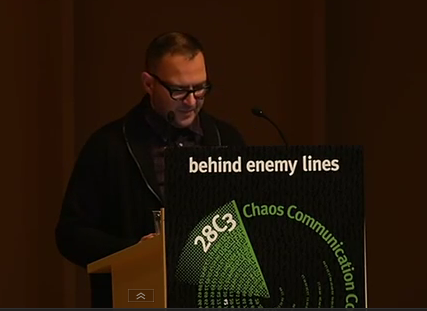
\includegraphics[width=0.8\textwidth]{images/chapter1/1-1}
  \caption[Cory Doctorow]{Ο Cory Doctorow παρουσιάζει την ομιλία του “Coming
War on General Computation” στο Chaos Communication Congress. Αξίζει να τη
δείτε και να την εμπεδώσετε:\\ \url{http://www.youtube.com/watch?v=yYqkU1y0AYc}}
  \label{1-1}
\end{figure}

\section{Στην Αρχή\ldots}
%
Οχι φυσικά, τα πράγματα δεν ήταν πάντα έτσι!  Γιατί απλά, το PC με τη μορφή
που ξέρετε σήμερα δεν υπήρχε στη δεκαετία του 80. Η για να το πούμε
διαφορετικά το ΙΒΜ PC αν και φτιάχτηκε κάπου τότε, απευθύνονταν μόνο σε
επιχειρήσεις και φυσικά η τιμή του ήταν αντίστοιχη. Ήταν ένα ιδιαίτερα
βαρετό μηχάνημα, χωρίς ήχο, με ασπρόμαυρη, πράσινη ή πορτοκαλί (!) οθόνη και
είχε τόσο ενδιαφέρον όσο ένα ντοκιμαντέρ της τηλεόρασης που το βλέπετε σε
εκατοστή επανάληψη στις πέντε το πρωί. Βέβαια το μηχάνημα αυτό δεν είχε τους
σημερινούς τεχνητούς περιορισμούς στον προγραμματισμό του, αλλά μη ξεχνάτε
δεν ήταν διαδεδομένο στους χομπίστες της εποχής αλλά στις εταιρίες.

Και όλοι εμείς που ξεκινήσαμε στα 80s τι χρησιμοποιούσαμε; Υπήρχε μια
ολόκληρη γενιά μηχανημάτων με τα οποία μεγάλωσαν πολλοί από τους
προγραμματιστές των οποίων τα προγράμματα χρησιμοποιείτε και σήμερα. Στις
εικόνες \ref{1-2}, \ref{1-3} και \ref{1-4} θα δείτε μερικά χαρακτηριστικά
μηχανήματα. Μπορείτε επίσης να επισκεφτείτε το προσωπικό μου\ldots{} μουσείο:\\
\url{http://museum.freebsdgr.org}

\begin{SCfigure}
  \centering
  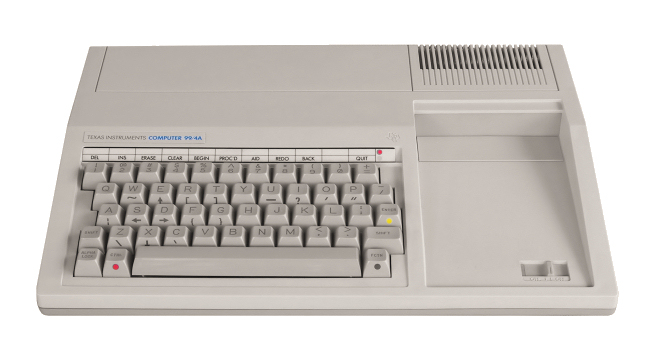
\includegraphics[width=0.60\textwidth]{images/chapter1/ti99}
  \caption[TI-99/4A]{Texas Instruments 99/4A. Γνωστό ως TI-99/4A. Αν δεν είχα τόσους servers ενεργούς 24/7, πιστεύω ότι αυτό (το πρώτο μου) μηχάνημα θα είχε
ρεκόρ\ldots{} uptime. Ναι, λειτουργεί ακόμα.\\
\url{http://www.youtube.com/watch?v=b2aXw7xWzgQ}}
  \label{1-2}
\end{SCfigure}

\begin{SCfigure}
  \centering
  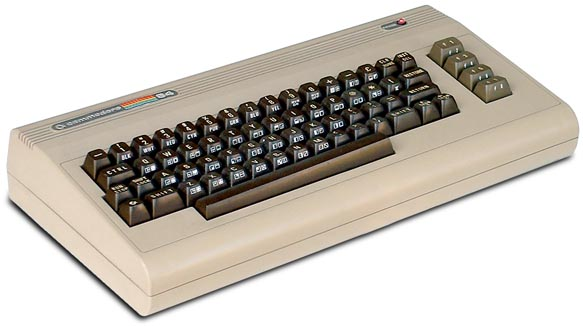
\includegraphics[width=0.60\textwidth]{images/chapter1/commodore64}
  \caption[Commodore 64]{Commodore 64, το μηχάνημα με το ρεκόρ πωλήσεων όλων των εποχών!  Και τώρα η (νέα) Commodore το ξαναβγάζει. Αλλά με i7 μέσα. Αν του τρέξετε Windows θα το θεωρήσω ιεροσυλία!}
  \label{1-3}
\end{SCfigure}

\begin{figure}
  \centering
  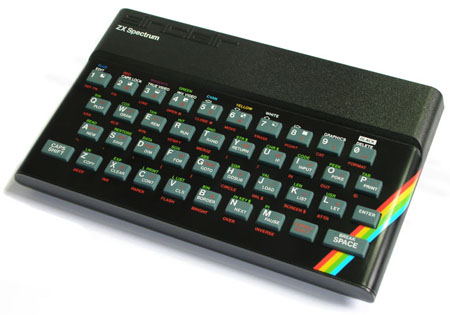
\includegraphics[width=0.8\textwidth]{images/chapter1/zxspectrum}
  \caption[Sinclair ZX Spectrum]{Sinclair ZX Spectrum, το γνωστό μηχάνημα με τις γομολάστιχες πλήκτρα! Πολύ γνωστό καθώς ήταν και σε προσιτή τιμή.}
  \label{1-4}
\end{figure}

Κοινό χαρακτηριστικό όλων των παραπάνω μηχανημάτων:
%
\begin{itemize}
\item[-] Το μόνο έτοιμο πρόγραμμα που είχαν ενσωματωμένο, ήταν μια γλώσσα
προγραμματισμού!
\end{itemize}
%
Κατά 99\%, ήταν μια διάλεκτος της γνωστής γλώσσας BASIC. Και αυτό που έκαναν
όλοι οι χομπίστες της εποχής, όλη μέρα, ήταν να γράφουν προγράμματα. Δικά
τους, από βιβλία, από περιοδικά. Ο προγραμματισμός βλέπετε είναι εθιστικός,
γιατί περιέχει μέσα την έννοια της δημιουργίας και τον έλεγχο του ανθρώπου
πάνω στη μηχανή. Κάτι που οι περισσότεροι έχουν εγκαταλείψει στις μέρες μας
(έχετε γράψει κάποιο πρόγραμμα για Windows;) και που τώρα οι εταιρίες
προσπαθούν να μας το απαγορέψουν έτσι και αλλιώς (βλέπε iPad).
%
\section{Είναι Αγγαρεία ο Προγραμματισμός;}
%
\subsection{Γιατί η Νέα Γενιά δεν Μαθαίνει Προγραμματισμό;}
%
Για διάφορους λόγους:
%
\begin{itemize}
\item Τα βρίσκει όλα έτοιμα.
\item Η πληροφορική έχει ταυτιστεί με τη διδασκαλία προγραμμάτων του τύπου
Word και Excel\ldots
\item Ας μπούμε καλύτερα στο Facebook/twitter/Google plus/YouNameIt social media να περάσουμε την ώρα μας.
\item Όχι, δεν θέλω άλλο να γράφω τα ακαταλαβίστικα που κάναμε στην Ανάπτυξη Εφαρμογών σε Προγραμματιστικό Περιβάλλον στο Λύκειο. Και δεν θέλω να ξαναδώ ποτέ την Γλώσσα!
\end{itemize}
%
\subsection{Γιατί οι Παλιοί Μάθαιναν Προγραμματισμό;}
%
\begin{itemize}
\item Δεν υπήρχε τίποτα έτοιμο. Έτσι και αλλιώς όποιος αγόραζε υπολογιστή είχε σκοπό να μάθει προγραμματισμό.
\item Η MS ήταν ένα μαγαζάκι σαν το εφημεριδοπωλείο της γωνίας και η επεξεργασία κειμένου γινόταν σε γραφομηχανές.
\item Το Internet ήταν καλά κρυμμένο στα όνειρα των BSDήδων που σχεδίαζαν το TCP/IP.
\item Όλοι εμείς που μαθαίναμε προγραμματισμό, το κάναμε γράφοντας ενδιαφέροντα προγράμματα: Με ήχο, γραφικά, κίνηση. Παιχνίδια!
\end{itemize}
%
Ο προγραμματισμός δεν μπορεί να είναι κάτι βαρετό. Σίγουρα, η αλγοριθμική
που κάνετε στο ΑΕΠΠ ή στον αντίστοιχο Δομημένο Προγραμματισμό των ΕΠΑΛ είναι
απαραίτητη. Αλλά δεν χρειάζεται όλα σας τα προγράμματα να υπολογίζουν
κλιμακωτές χρεώσεις σε λογαριασμούς ΔΕΗ και αθροίσματα αριθμών ``μέχρι να
δώσετε το μηδέν''. Έλεος πια! Ο προγραμματισμός έχει ρουτίνες, αλλά δεν
πρέπει με τίποτα να καταντάει για εμάς ρουτίνα. Game programming FTW!
%
\section{Καλώς Ήλθατε στην Python!}
%
Εντάξει, πειστήκατε. Θα δώσετε στον προγραμματισμό ακόμα μια ευκαιρία. Αρκεί
να μην έχει προγράμματα που θα αθροίζουν αριθμούς και λογαριασμούς ΔΕΗ. Βέβαια,
δεν γίνεται να ξεκινήσουμε από το μηδέν γράφοντας killer προγράμματα. Σας
υποσχόμαστε όμως ότι θα προσπαθήσουμε να πάμε στο στόχο μας σχετικά γρήγορα
και με όσο το δυνατόν πιο ενδιαφέροντα προγράμματα.

Το όχημα μας σε αυτή την αναζήτηση θα είναι η γλώσσα python. Την επιλέξαμε
επειδή:
%
\begin{itemize}
\item Είναι κατάλληλη για εκμάθηση ως πρώτη γλώσσα προγραμματισμού.
\item Είναι πολύ ισχυρή -- παρέχει τόσες έτοιμες βιβλιοθήκες (python modules) που μας επιτρέπουν να κάνουμε τα πάντα.
\item Τρέχει σε οτιδήποτε σχεδόν μπορείτε να φανταστείτε. Ναι, ακόμα και στο iPad σας. Στο PC σας. Στα Windows. Στο Linux. Στο FreeBSD.
\item Παρέχει εκείνη την ωραία αμεσότητα της BASIC των 80s!
\end{itemize}
%
\subsection{Εγκατάσταση της Python}
%
Αν χρησιμοποιείτε Linux ή FreeBSD ενδεχομένως την έχετε ήδη εγκατεστημένη.
Αν όχι, εγκαταστήστε την python2.7 από το repository της διανομής σας. Π.χ.
σε debianoειδή λειτουργικά θα χρειαστεί να γράψετε κάτι σαν:
%
\begin{verbatim}
# apt-get install python2.7
\end{verbatim}
%
Στο FreeBSD μπορείτε να κάνετε εγκατάσταση από το port:
%
\begin{verbatim}
# cd /usr/ports/lang/python27
# make install clean
\end{verbatim}
%
Στα Windows, κατεβάστε την από τη σελίδα
\url{http://www.python.org/download/releases}. Κατεβάστε και εγκαταστήστε την
τελευταία έκδοση της σειράς 2.7 για συμβατότητα με αυτά που θα φτιάχνουμε
εδώ.
%
\subsection{Τα Πρώτα σας Πειράματα στην Python}
%
H python έρχεται με ένα περιβάλλον άμεσης εκτέλεσης εντολών το {\em idle}, το
οποίο μπορείτε να το εκτελέσετε γράφοντας απλώς idle ή επιλέγοντας το από το
μενού του λειτουργικού σας. Ακόμα και αν δεν έχετε το idle, μπορείτε να
γράψετε στη γραμμή εντολών:
%
\begin{verbatim}
$ python
\end{verbatim}
%
το οποίο πάλι θα ξεκινήσει την python σε κατάσταση άμεσης εκτέλεσης εντολών.
Γράψτε {\tt exit()} για να τερματίσετε. Σε κάθε περίπτωση θα δείτε κάτι σαν το
παρακάτω:
%
\begin{verbatim}
Python 2.7.2 (default, Jun 12 2011, 14:24:46)
Type "copyright", "credits" or "license()" for more information.
>>>
\end{verbatim}
%
Για αρχή, ας δοκιμάσουμε κάτι απλό. Στην απευθείας εκτέλεση εντολών μπορείτε
να κάνετε πράξεις απευθείας:

\begin{minted}[bgcolor=bg,  frame=lines, framesep=10pt]{python}
>>> 4/2
2

>>> 5*3
15

>>> 1/2
0
\end{minted}

Μηδέν; Αν δεν το καταλάβατε, η διαίρεση που γίνεται είναι ακέραια, καθώς η
python βλέπει ότι τα ορίσματα είναι ακέραια.  Αν κάνετε ένα αριθμό δεκαδικό,
θα πάρετε την απάντηση που περιμένατε:

\begin{minted}[bgcolor=bg,  frame=lines, framesep=10pt]{python}
>>> 1/2.0
0.5
\end{minted}

Το υπόλοιπο της διαίρεσης, ο γνωστός τελεστής mod, στην python είναι το \%:

\begin{minted}[bgcolor=bg,  frame=lines, framesep=10pt]{python}
>>> 1 % 2
1

>>> 5 % 3
2
\end{minted}

Ενώ αν θέλετε να υψώσετε ένα αριθμό σε μια δύναμη:

\begin{minted}[bgcolor=bg,  frame=lines, framesep=10pt]{python}
>>> 2**24

16777216
\end{minted}

Ακόμα πιο ενδιαφέρον, είναι ότι η python μπορεί να κάνει απευθείας πράξεις
σε δεκαεξαδικό, οκταδικό και δυαδικό. Για δεκαεξαδικό, γράψτε τον αριθμό
ξεκινώντας με {\bf 0x} και για δυαδικό με {\bf 0b}:

\begin{minted}[bgcolor=bg,  frame=lines, framesep=10pt]{python}
>>> 0xFF
255

>>> 0b1100
12
\end{minted}
%
\subsection{Μεταβλητές}
%
Όπως πιθανώς θα ξέρετε, μια μεταβλητή είναι ένα όνομα που αντιπροσωπεύει μια
τιμή. Χρησιμοποιώντας μεταβλητές είναι δυνατόν να φτιάξουμε προγράμματα που
λύνουν ένα πρόβλημα με γενικό τρόπο, αφού μπορούμε να αλλάζουμε την τιμή
τους σε κάθε εκτέλεση του προγράμματος. Για παράδειγμα:

\begin{minted}[bgcolor=bg,  frame=lines, framesep=10pt]{python}
>>> a=5
>>> a*5
25
>>> a**3
125
\end{minted}
%
\subsection{Είσοδος από το Χρήστη και Εμφάνιση στην Οθόνη}
%
Με την {\tt input} μπορούμε να ζητήσουμε από το χρήστη μια τιμή την ώρα που το
πρόγραμμα εκτελείται. Η τιμή αυτή μπορεί να αποθηκευθεί απευθείας σε μια
μεταβλητή όπως φαίνεται παρακάτω:

\begin{minted}[bgcolor=bg,  frame=lines, framesep=10pt]{python}
>>> age=input("What is your age? ")
What is your age? 24
>>> print age
24
\end{minted}

Όπως καταλάβατε, η εντολή {\tt print} χρησιμοποιείται για να τυπώσουμε κάτι στην
οθόνη. Μπορεί να είναι ένα μήνυμα (σε εισαγωγικά), μια τιμή, ή μια
μεταβλητή. Ή και συνδυασμός των παραπάνω:

\begin{minted}[bgcolor=bg,  frame=lines, framesep=10pt]{python}
>>> print age,"is not too bad!"
24 is not too bad!
\end{minted}
%
\subsection{Το Πρώτο σας Πρόγραμμα: HelloWorld!}
%
Εντάξει, μια πιο καλή παραλλαγή έστω. Αν χρησιμοποιείτε το {\tt idle}, επιλέξτε
από το μενού {\tt File => New Window} για να βρεθείτε σε ένα απλό editor. Αλλά
μπορείτε να χρησιμοποιήσετε και όποιο άλλο text editor θέλετε. Γράψτε:

\begin{minted}[bgcolor=bg, linenos, frame=lines, framesep=10pt]{python}
name=raw_input("What is your name? ")
age=input("What is your age? ")
print "Pleased to meet you ",name
print age, " is not too bad!"
\end{minted}

Αποθηκεύστε το ως {\tt hello.py}. Στο {\tt idle}, απλά πιέστε {\tt F5} για να εκτελεστεί το πρόγραμμα.  Σε UNIXoειδή λειτουργικά, μπορείτε επίσης να το τρέξετε από το τερματικό:
%
\begin{verbatim}
$ python hello.py
\end{verbatim}
%
Τι είναι το {\tt raw\_input}; Πειραματιστείτε βάζοντας σκέτο {\tt input} και δείτε τι θα γίνει. Μετά, δώστε το όνομα σας σε εισαγωγικά. Μπορείτε να βρείτε γιατί
συμβαίνει αυτό; Θα το δούμε στη συνέχεια του κεφαλαίου.

Ας γράψουμε τώρα το πρώτο μας text παιχνίδι\ldots
%
\section{Το Πρώτο Σας Παιχνίδι: Βρες τον Αριθμό}
%
Γράψτε το παρακάτω και αποθηκεύστε το ως {\tt guess.py} ή όπως αλλιώς θέλετε.
Εκτελέστε το όπως προηγουμένως.

\begin{minted}[bgcolor=bg, linenos, frame=lines, framesep=10pt]{python}
#
# Βρες τον αριθμό. Απόπειρα 1
#
import random
thenumber = random.randint(1,50)
print "Έχω σκεφτεί ένα αριθμό από το 1 ως το 50."
print "Μπορείς να τον βρεις;"
guess = 0
while guess != thenumber:
  guess = input("Δώσε τον αριθμό: ")
  if guess > thenumber:
    print "Έδωσες μεγαλύτερο αριθμό!"
  if guess < thenumber:
    print "Έδωσες μικρότερο αριθμό!"
  if guess == thenumber:
    print "Τον βρήκες!!!"
\end{minted}

Προσοχή! Τα κενά είναι σημαντικά. Η python δεν έχει άγκιστρα, αγκύλες ή
οτιδήποτε άλλο χρησιμοποιούν οι άλλες γλώσσες για να ξεχωρίζουν ποιες
εντολές ανήκουν σε μια {\em σύνθετη εντολή}. Αντίθετα, χρησιμοποιεί τα κενά
ή τα tabs για τον ίδιο σκοπό. Δείτε για παράδειγμα ότι όλες οι εντολές
κάτω από τη {\tt while} είναι δύο κενά διαστήματα πιο μέσα: σημαίνει ότι όλες
ανήκουν στη {\tt while}. Κάτω από κάθε {\tt if}, η εντολή είναι δύο διαστήματα πιο μέσα: ανήκει στην {\tt if}. Σε όλες πρακτικά τις γλώσσες πρέπει να στοιχίζουμε το πρόγραμμα μας σωστά ώστε να είναι ευανάγνωστο. Απλώς στην python αυτό είναι
υποχρεωτικό καθώς η στοίχιση είναι μέρος του συντακτικού της γλώσσας!
%
\subsection{Ανάλυση Γραμμή -- Γραμμή}
%
\begin{minted}[bgcolor=bg,  frame=lines, framesep=10pt]{python}
import random
\end{minted}

Δηλώνουμε στην python ότι θέλουμε να χρησιμοποιήσουμε τη βιβλιοθήκη (module)
{\tt random}. Μέσα σε αυτή περιέχονται συναρτήσεις που παράγουν τυχαίους αριθμούς!

\begin{minted}[bgcolor=bg,  frame=lines, framesep=10pt]{python}
thenumber = random.randint(1,50)
\end{minted}

Χρησιμοποιούμε την {\tt randint} για να παράγουμε ένα ακέραιο τυχαίο αριθμό
από το 1 ως το 50 και τον αποθηκεύουμε στη μεταβλητή {\tt thenumber}.
Παρατηρήστε πως καλούμε τη συνάρτηση {\tt randint}.

\begin{minted}[bgcolor=bg,  frame=lines, framesep=10pt]{python}
print "Έχω σκεφτεί ένα αριθμό από το 1 ως το 50."
print "Μπορείς να τον βρεις;"
\end{minted}

Τα γνωστά μηνύματα, δεν χρειάζονται εξήγηση.

\begin{minted}[bgcolor=bg,  frame=lines, framesep=10pt]{python}
guess = 0
\end{minted}

Η αρχική μας πρόβλεψη. Η μεταβλητή {\tt guess} θα κρατάει τον αριθμό που
δίνουμε κάθε φορά ως μαντεψιά. Της δίνουμε μια αρχική τιμή 0 ώστε σίγουρα
να μην ανήκει στο διάστημα 1 ως 50 που παράγει το πρόγραμμα. Έτσι
εξασφαλίζουμε ότι η επόμενη εντολή:

\begin{minted}[bgcolor=bg,  frame=lines, framesep=10pt]{python}
while guess != thenumber:
\end{minted}

Θα εκτελεστεί, καθώς λέει: ``Κάνε τα παρακάτω, όσο ο αριθμός που έδωσε ο
χρήστης δεν είναι ίδιος (!=) με αυτό που σκέφτηκε η {\tt randint}''. Και καθώς η
αρχική τιμή είναι το μηδέν, σίγουρα το πρόγραμμα θα προχωρήσει:

\begin{minted}[bgcolor=bg,  frame=lines, framesep=10pt]{python}
  guess = input("Δώσε τον αριθμό: ")
\end{minted}

Ζητάει τον αριθμό από τον παίκτη.

\begin{minted}[bgcolor=bg,  frame=lines, framesep=10pt]{python}
  if guess > thenumber:
    print "Έδωσες μεγαλύτερο αριθμό!"
\end{minted}

Αν ο χρήστης έδωσε μεγαλύτερο αριθμό, τυπώνεται το αντίστοιχο μήνυμα.

\begin{minted}[bgcolor=bg,  frame=lines, framesep=10pt]{python}
  if guess < thenumber:
    print "Έδωσες μικρότερο αριθμό!"
\end{minted}

Αν ο χρήστης έδωσε μικρότερο αριθμό, τυπώνεται πάλι αντίστοιχο μήνυμα.

\begin{minted}[bgcolor=bg,  frame=lines, framesep=10pt]{python}
  if guess == thenumber:
    print "Τον βρήκες!!!"
\end{minted}

Αν ο χρήστης βρήκε τον αριθμό, τυπώνεται το\ldots{} νικητήριο μήνυμα.
Παρατηρήστε ότι ο έλεγχος ισότητας γίνεται με δύο ίσον (==). Το ένα ίσον
χρησιμοποιείται για να δώσουμε τιμή σε μεταβλητή.

Σε όλες τις περιπτώσεις, το πρόγραμμα επιστρέφει στην {\tt while} όπου
ξεκίνησε.  Αν όμως ο αριθμός που έδωσε ο χρήστης είναι ίσος με το
{\tt thenumber}, η συνθήκη δεν ισχύει πλέον και το πρόγραμμα τερματίζει.

Ξαναδιαβάστε τώρα το πρόγραμμα προσεκτικά. Βλέπετε κάτι να περιττεύει;
Αν όχι σκεφτείτε λίγο το τελευταίο {\tt if}. Χρειάζεται στα αλήθεια; Καθώς
ο βρόχος {\tt while} τερματίζει μόνο όταν ο παίκτης βρει τον αριθμό, το
τελευταίο if μπορεί να παραλειφθεί εντελώς, και το μήνυμα επιτυχίας
να μπει μόνο του, αμέσως μετά το βρόχο. Φτάνουμε έτσι στην Απόπειρα 2
του προγράμματος:

\begin{minted}[bgcolor=bg, linenos, frame=lines, framesep=10pt]{python}
#
# Βρες τον αριθμό. Απόπειρα 2
#
import random
thenumber = random.randint(1,50)
print "Έχω σκεφτεί ένα αριθμό από το 1 ως το 50."
print "Μπορείς να τον βρεις;"
guess = 0
while guess != thenumber:
  guess=input("Δώσε τον αριθμό: ")
  if guess > thenumber:
    print "Έδωσες μεγαλύτερο αριθμό!"
  if guess < thenumber:
    print "Έδωσες μικρότερο αριθμό!"
print "Τον βρήκες!!!"
\end{minted}
%
%
\section{Επεκτείνοντας το Παιχνίδι}
%
Ακολουθούν μερικές βελτιώσεις για το απλό μας παιχνίδι -- στην πραγματικότητα μια ευκαιρία να μάθουμε μερικά ακόμα στοιχεία της python!
%
\subsection{Όνομα Χρήστη και Νικητήριο Μήνυμα}
%
Μπορούμε εύκολα να επεκτείνουμε το παιχνίδι μας ώστε να ρωτάει το χρήστη το όνομα του στην αρχή και να το εμφανίζει στο νικητήριο μήνυμα: ``Συγχαρητήρια Γιώργο το βρήκες!''

Πολύ απλό νομίζουμε, αρκεί να βάλετε την παρακάτω γραμμή πριν από το πρώτο {\tt print}:

\begin{minted}[bgcolor=bg,  frame=lines, framesep=10pt]{python}
name = input("Δώσε το όνομα σου: ")
\end{minted}

Και να αλλάξετε την τελευταία γραμμή σε:

\begin{minted}[bgcolor=bg,  frame=lines, framesep=10pt]{python}
print "Συγχαρητήρια", name, "τον βρήκες!"
\end{minted}

Για εκτελέστε το όμως! Θα διαπιστώσετε με έκπληξη ότι δεν δέχεται το όνομα
σας, εκτός αν το δώσετε μέσα σε εισαγωγικά. Όχι, δεν είναι ότι η python
έχει προσωπικά μαζί σας. Απλώς η εντολή {\tt input} ερμηνεύει την είσοδο ως
παράσταση και ψάχνει να βρει το όνομα σας ως κάτι που έχει ήδη οριστεί στο
πρόγραμμα! Αν δώσετε ως όνομα το {\tt thenumber}, μεταβλητή που ήδη έχει ορισθεί στο πρόγραμμα μας, η python θα το δεχθεί. Δοκιμάστε και θα δείτε το αποτέλεσμα!

Φυσικά, αυτό δεν είναι κάτι που θέλουμε. Και ούτε μας αρέσει η ιδέα να
βάζουμε εισαγωγικά γύρω από το όνομα μας ή οποιοδήποτε αλφαριθμητικό θέλουμε
να δώσουμε στην είσοδο.  Η λύση σε αυτό είναι η {\tt raw\_input}:

\begin{minted}[bgcolor=bg,  frame=lines, framesep=10pt]{python}
name = raw_input("Δώσε το όνομα σου: ")
\end{minted}

Θα χρησιμοποιούμε από εδώ και πέρα την {\tt raw\_input} για είσοδο αλφαριθμητικών
%
\subsection{Προσθήκη Μετρητή Προσπαθειών}
%
Θα προσθέσουμε μια μεταβλητή {\tt count} στην οποία θα δώσουμε αρχικά τιμή 0
και κάθε φορά που ο χρήστης θα δίνει ένα αριθμό θα αυξάνει κατά 1 ({\tt
count = count + 1}). Όταν ο χρήστης βρει τον αριθμό, το πρόγραμμα θα τυπώνει και πόσες προσπάθειες χρειάστηκε.

Και αυτό είναι αρκετά εύκολο. Δείτε την πλήρη τρίτη εκδοχή του προγράμματος:

\begin{minted}[bgcolor=bg, linenos, frame=lines, framesep=10pt]{python}
#
# Βρες τον αριθμό. Απόπειρα 3
#
import random
thenumber = random.randint(1,50)
name = raw_input("Δώσε το όνομα σου: ")
print "Έχω σκεφτεί ένα αριθμό από το 1 ως το 50."
print "Μπορείς να τον βρεις;"
guess = 0
tries = 0
while guess != thenumber:
  tries = tries + 1
  guess=input("Δώσε τον αριθμό: ")
  if guess > thenumber:
    print "Έδωσες μεγαλύτερο αριθμό!"
  if guess < thenumber:
    print "Έδωσες μικρότερο αριθμό!"
print "Συγχαρητήρια", name, "τον βρήκες σε", tries, "προσπάθειες!"
\end{minted}

Η γραμμή που αυξάνει τη μεταβλητή {\tt tries} μπορεί να γραφεί και έτσι:

\begin{minted}[bgcolor=bg,  frame=lines, framesep=10pt]{python}
  tries += 1
\end{minted}

Είναι μια συντομογραφία που θα συναντήσετε συχνά. Φυσικά το ίδιο μπορεί να γίνει και με τους άλλους αριθμητικούς τελεστές (για αφαίρεση, πολλαπλασιασμό κλπ)
αλλά το παραπάνω είναι το πιο συχνό.
%
\subsection{Κριτική στην\ldots{} Ικανότητα του Παίκτη}
%
Θα επεκτείνουμε το πρόγραμμα ώστε αν ο χρήστης βρεί τον αριθμό σε μια προσπάθεια θα του τυπώνει το μήνυμα ``Beginner's luck!'', αν το βρει σε πέντε ή λιγότερες προσπάθειες το μήνυμα ``Είσαι γρήγορος'' και αν το βρει σε πάνω από πέντε, το μήνυμα ``Η γιαγιά μου παίζει πιο καλά!''

Μια πρώτη σκέψη ίσως είναι αυτή (οι γραμμές
φυσικά μπαίνουν στο τέλος):

\begin{minted}[bgcolor=bg, linenos, frame=lines, framesep=10pt]{python}
if tries == 1:
  print "Beginner's luck!"
if tries <= 5:
  print "Είσαι γρήγορος!"
if tries > 5:
  print "Η γιαγιά μου παίζει πιο καλά!"
\end{minted}

Έχουμε λίγες γραμμές κώδικα, και ήδη έχουμε bugs. Αν βρείτε τον
αριθμό σε μια προσπάθεια, θα πάρετε δύο μηνύματα! ``Beginner's luck'' και
``Είσαι γρήγορος!'' Φυσικά, καθώς το 1 είναι επίσης και μικρότερο από 5,
εκτελούνται δύο εντολές {\tt if}. Εδώ υπάρχουν δύο πιθανές λύσεις:
%
\begin{itemize}
\item Να αλλάξουμε τη δεύτερη συνθήκη ώστε να εκτελείται όταν η
            {\tt tries} είναι μικρότερη από 5 και ταυτόχρονα διαφορετική του 1
            (ή μεγαλύτερη του 1)
\item Να φτιάξουμε την {\tt if} με τέτοιο τρόπο ώστε αν εκτελεστεί μια
            συνθήκη να μην εκτελείται καμιά άλλη.
\end{itemize}
%
Θα μπορούσαμε να το γράψουμε έτσι:

\begin{minted}[bgcolor=bg, linenos, frame=lines, framesep=10pt]{python}
if tries == 1:
  print "Beginners luck!"
if (tries <= 5 and tries != 1):
  print "Είσαι γρήγορος!"
if tries > 5:
  print "Η γιαγιά μου παίζει πιο καλά!"
\end{minted}

Φτιάξαμε εδώ μια σύνθετη συνθήκη χρησιμοποιώντας τον λογικό τελεστή {\tt and}
o οποίος πρακτικά σημαίνει ότι θα είναι αληθής και θα
εκτελεστεί μόνο αν συμβαίνουν και τα δύο μέρη: και το {\tt tries} να είναι
μικρότερο ή ίσο από 5 και διαφορετικό από το 1 (θα μπορούσατε επίσης να
το γράψετε και μεγαλύτερο από το 1). Καθώς φαντάζεστε υπάρχουν και οι
λογικοί τελεστές {\tt or} και {\tt not} που θα δούμε σε παραδείγματα αργότερα.

Ένας άλλος τρόπος είναι να χρησιμοποιήσουμε μια πιο πλήρη μορφή της {\tt if},
που περιέχει επίσης τo {\tt elif} ({\em else if}, αλλιώς αν) και το {\tt else}:

\begin{minted}[bgcolor=bg, linenos, frame=lines, framesep=10pt]{python}
if tries == 1:
  print "Beginners luck!"
elif tries <= 5:
  print "Είσαι γρήγορος!"
else:
  print "Η γιαγιά μου παίζει πιο καλά!"
\end{minted}

Εδώ η συνθήκη που βρίσκεται στο {\tt elif} (αλλιώς αν) θα εκτελεστεί μόνο αν το {\tt tries} είναι μικρότερο του 5, και δεν έχει εκτελεστεί το πρώτο {\tt if}. H δομή της {\tt if-elif} εξασφαλίζει ότι μόλις εκτελεστεί μια οποιαδήποτε από τις συνθήκες (είτε ή {\tt if}, είτε κάποια από τις {\tt elif} - και μπορούμε να βάλουμε πολλές {\tt elif}) οι υπόλοιπες περιπτώσεις δεν εξετάζονται. Αν υπάρχουν εντολές κάτω από τη δομή {\tt if-elif-else}, η εκτέλεση θα συνεχιστεί από εκεί. Καθώς φαντάζεστε, η εντολή {\tt else} εκτελείται μόνο όταν δεν εκτελεστεί καμιά από τις {\tt elif} ή η αρχική {\tt if}.

Μπορείτε να βρείτε το πλήρες πρόγραμμα στο παράρτημα, σελ. \pageref{listing:guess}.
